\chapter{The Carey Foster Bridge}

\section*{Objectives}

\begin{enumerate}
\item To understand how a Carey Foster bridge works.
\item To find the value of an unknown low resistance using the Carey Foster bridge.
\end{enumerate}


\section*{Introduction}
\subsection*{Measurement of low resistance} 
Ohm's law, $V=IR$, states that the current flowing through a resistor with resistance $R$ varies linearly with the potential difference across it.
To measure the resistance, one method involves studying the IV characteristics of a resistor, i.e looking at the variation in the current, $I$, flowing through the resistor for a range of applied potential differences, $V$ and then extracting the value of the resistance, $R$, from the resulting graph/data. This direct application of Ohm's law usually works well for resistances in the range $1-100 \Omega$. 

\begin{figure}[!htb]
    \centering
    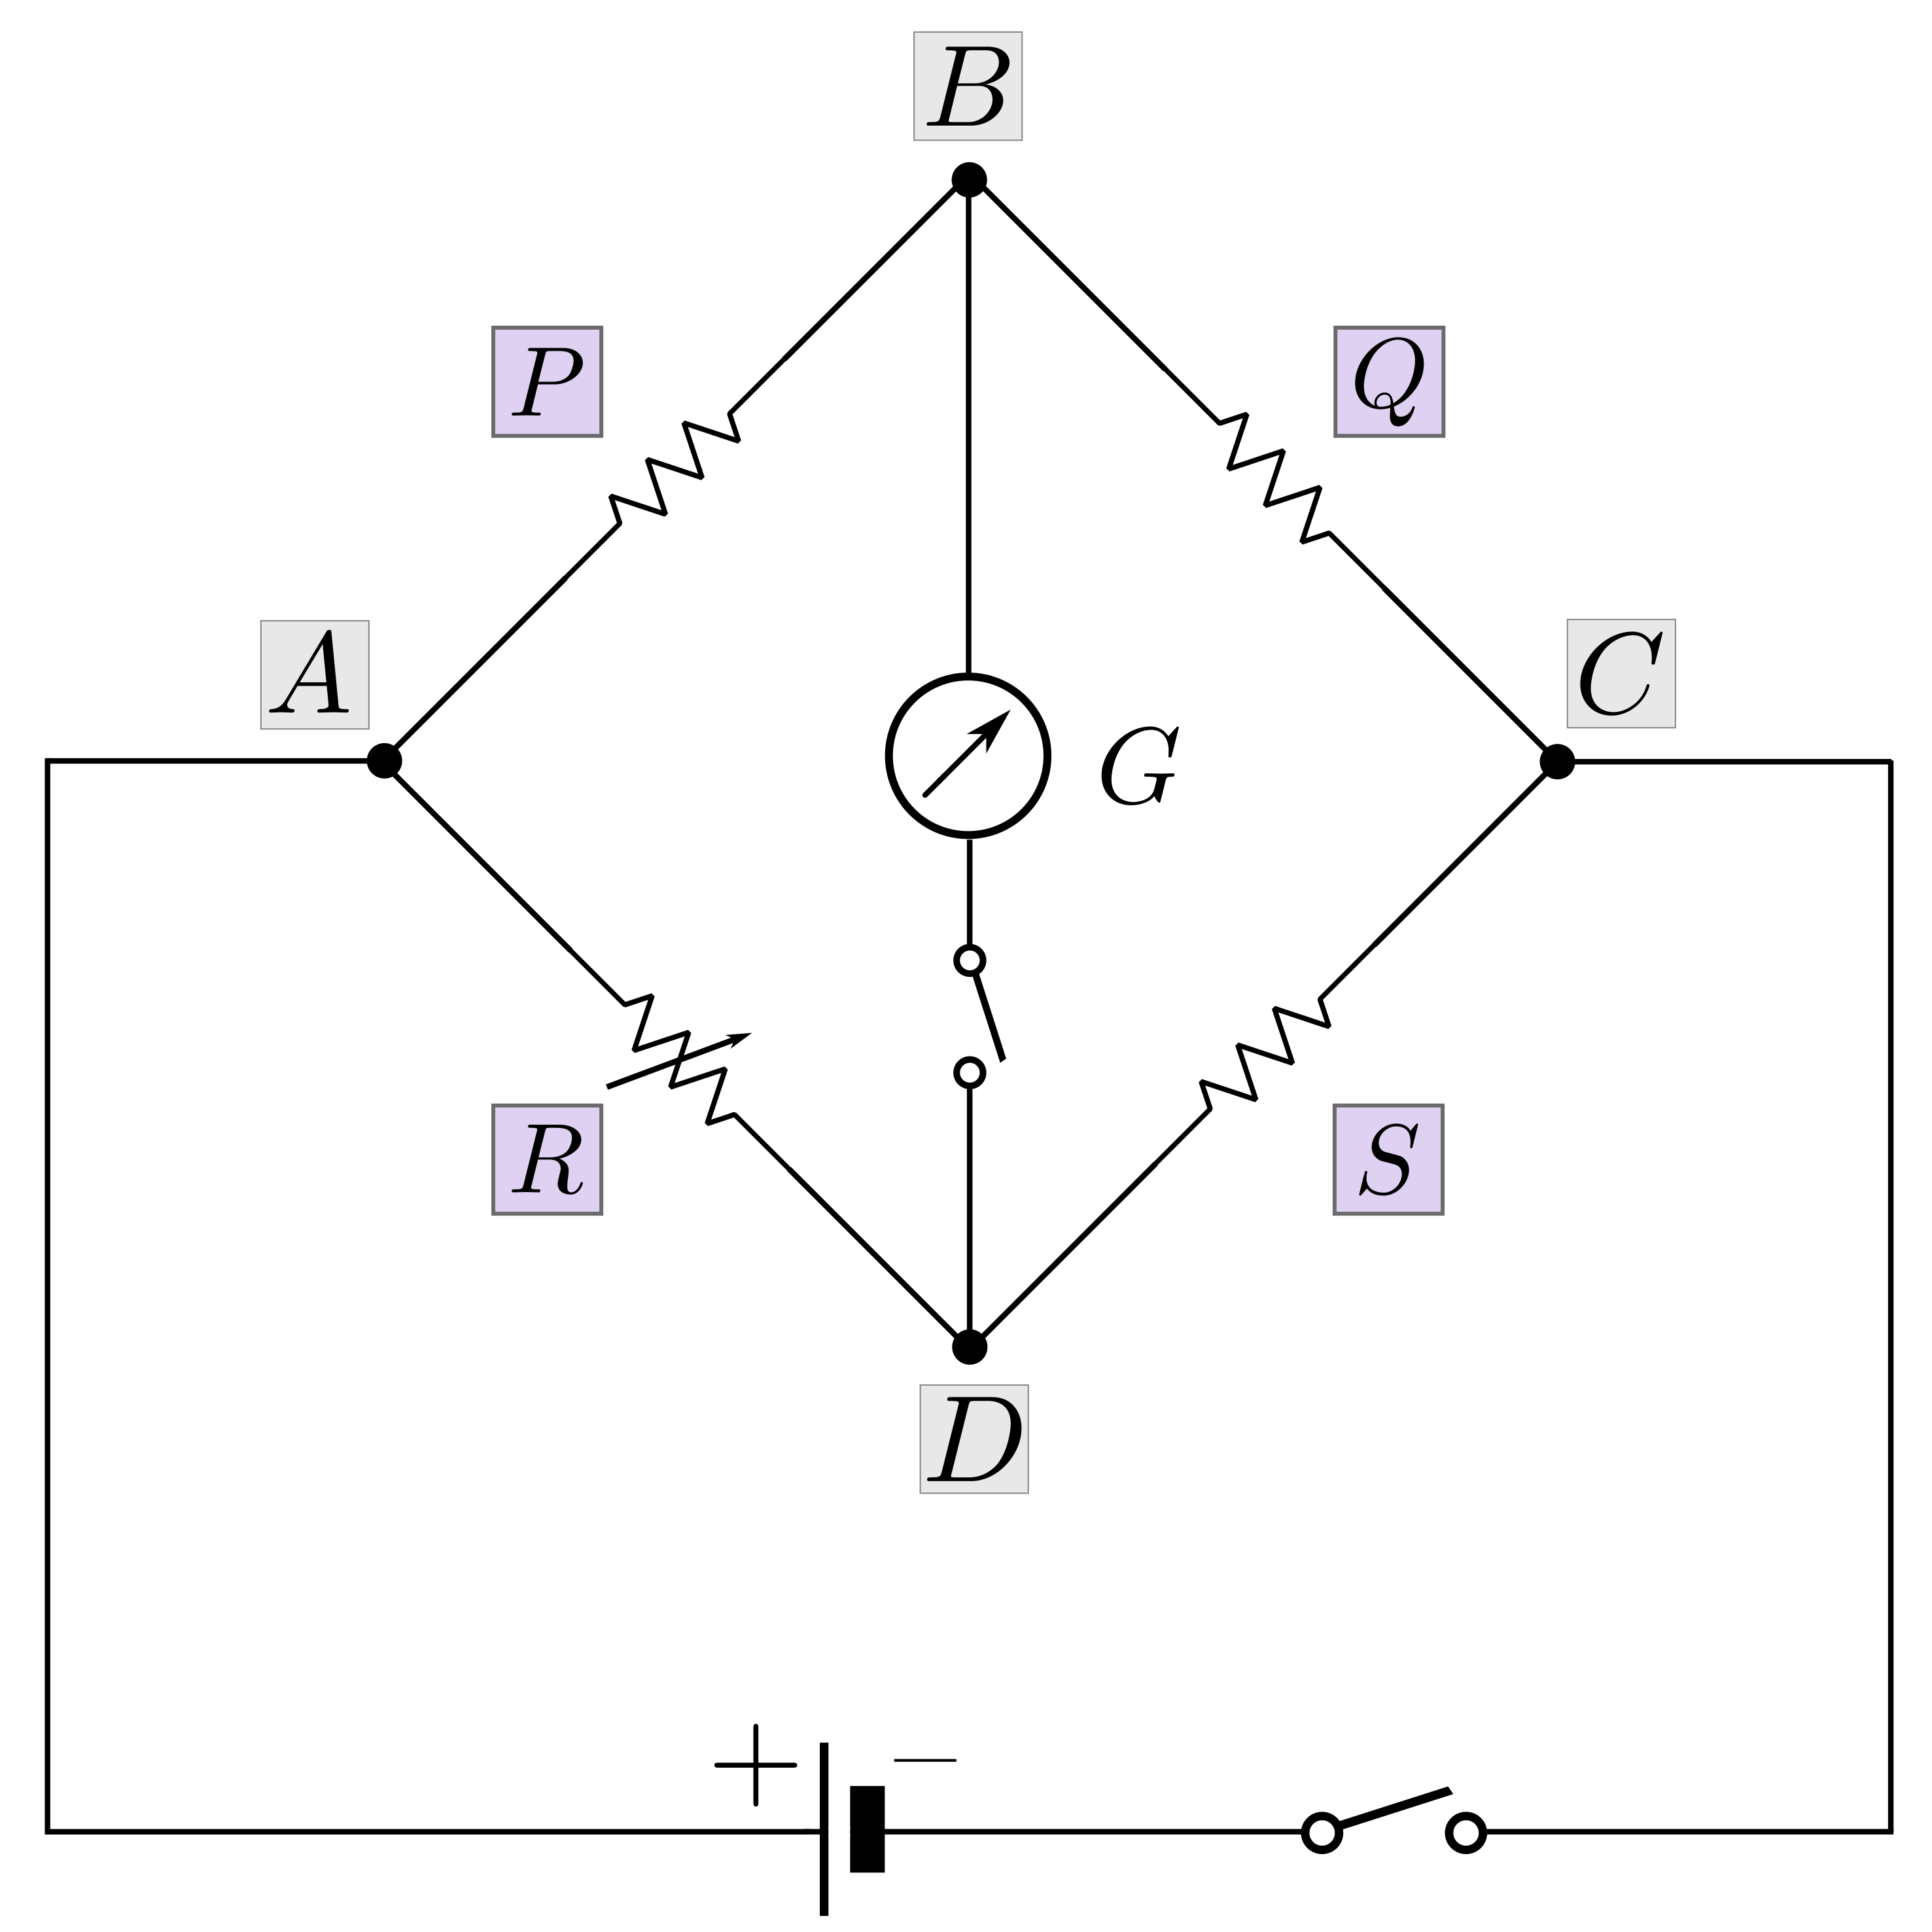
\includegraphics[width=0.5\textwidth]{figs/wheatstone.png}
    \caption{Schematic diagram of a Wheatstone bridge.}
    \label{fig:wheatstone}
\end{figure}

For the measurement of low resistances, it is preferable to use methods that work on comparison of resistances (so you would need, in the first place, some precisely known, standard resistances). Such methods are based on the principle of a Wheatstone's bridge. A Wheatstone bridge is shown in Figure (\ref{fig:wheatstone}). A current measuring device, the galvanometer, registers current flowing in the arm $BD$. However, when the nodes $B$ and $D$ are at the same potential, no current flows in the arm $BD$. This happens when the following relation between the resistances is satisfied
\begin{equation}
    \frac{P}{Q}  =\frac{R}{S}
    \label{balanceofthebridges}
\end{equation}
In such a situation, the Wheatstone bridge is said to be \textit{balanced}.
To find out the resistance of an unknown resistor, two standard resistors are wired in arms $AB$ and $BC$. The value of the (variable) resistor, $R$, is varied until the point of zero/null deflection/display is found on the galvanometer. Since, the bridge is now balanced, Equation (\ref{balanceofthebridges}) holds good, and we can infer the value of an unknown resistance, $S$. 

We note here that this null method, which hinges on balancing the Wheatstone bridge, is useful because by not measuring a finite value of the current, the galvanometer does not have any role to play in the accuracy of the resistance measurement, our measurement of an unknown low resistances is limited only by the precision of other resistors in the experimental setup. In this experiment, we will use a form of modified Wheatstone bridge called a Carey Foster bridge, which is useful to measure low resistances while eliminating end corrections.

% \section*{Description}

% In \textbf{Part A}, you will determine the apparent value of a small resistance. 

% In \textbf{Part B}, you will determine a small correction. 

%In \textbf{Part C}, 

\section*{Theory}

\begin{figure}[!htb]
    \centering
    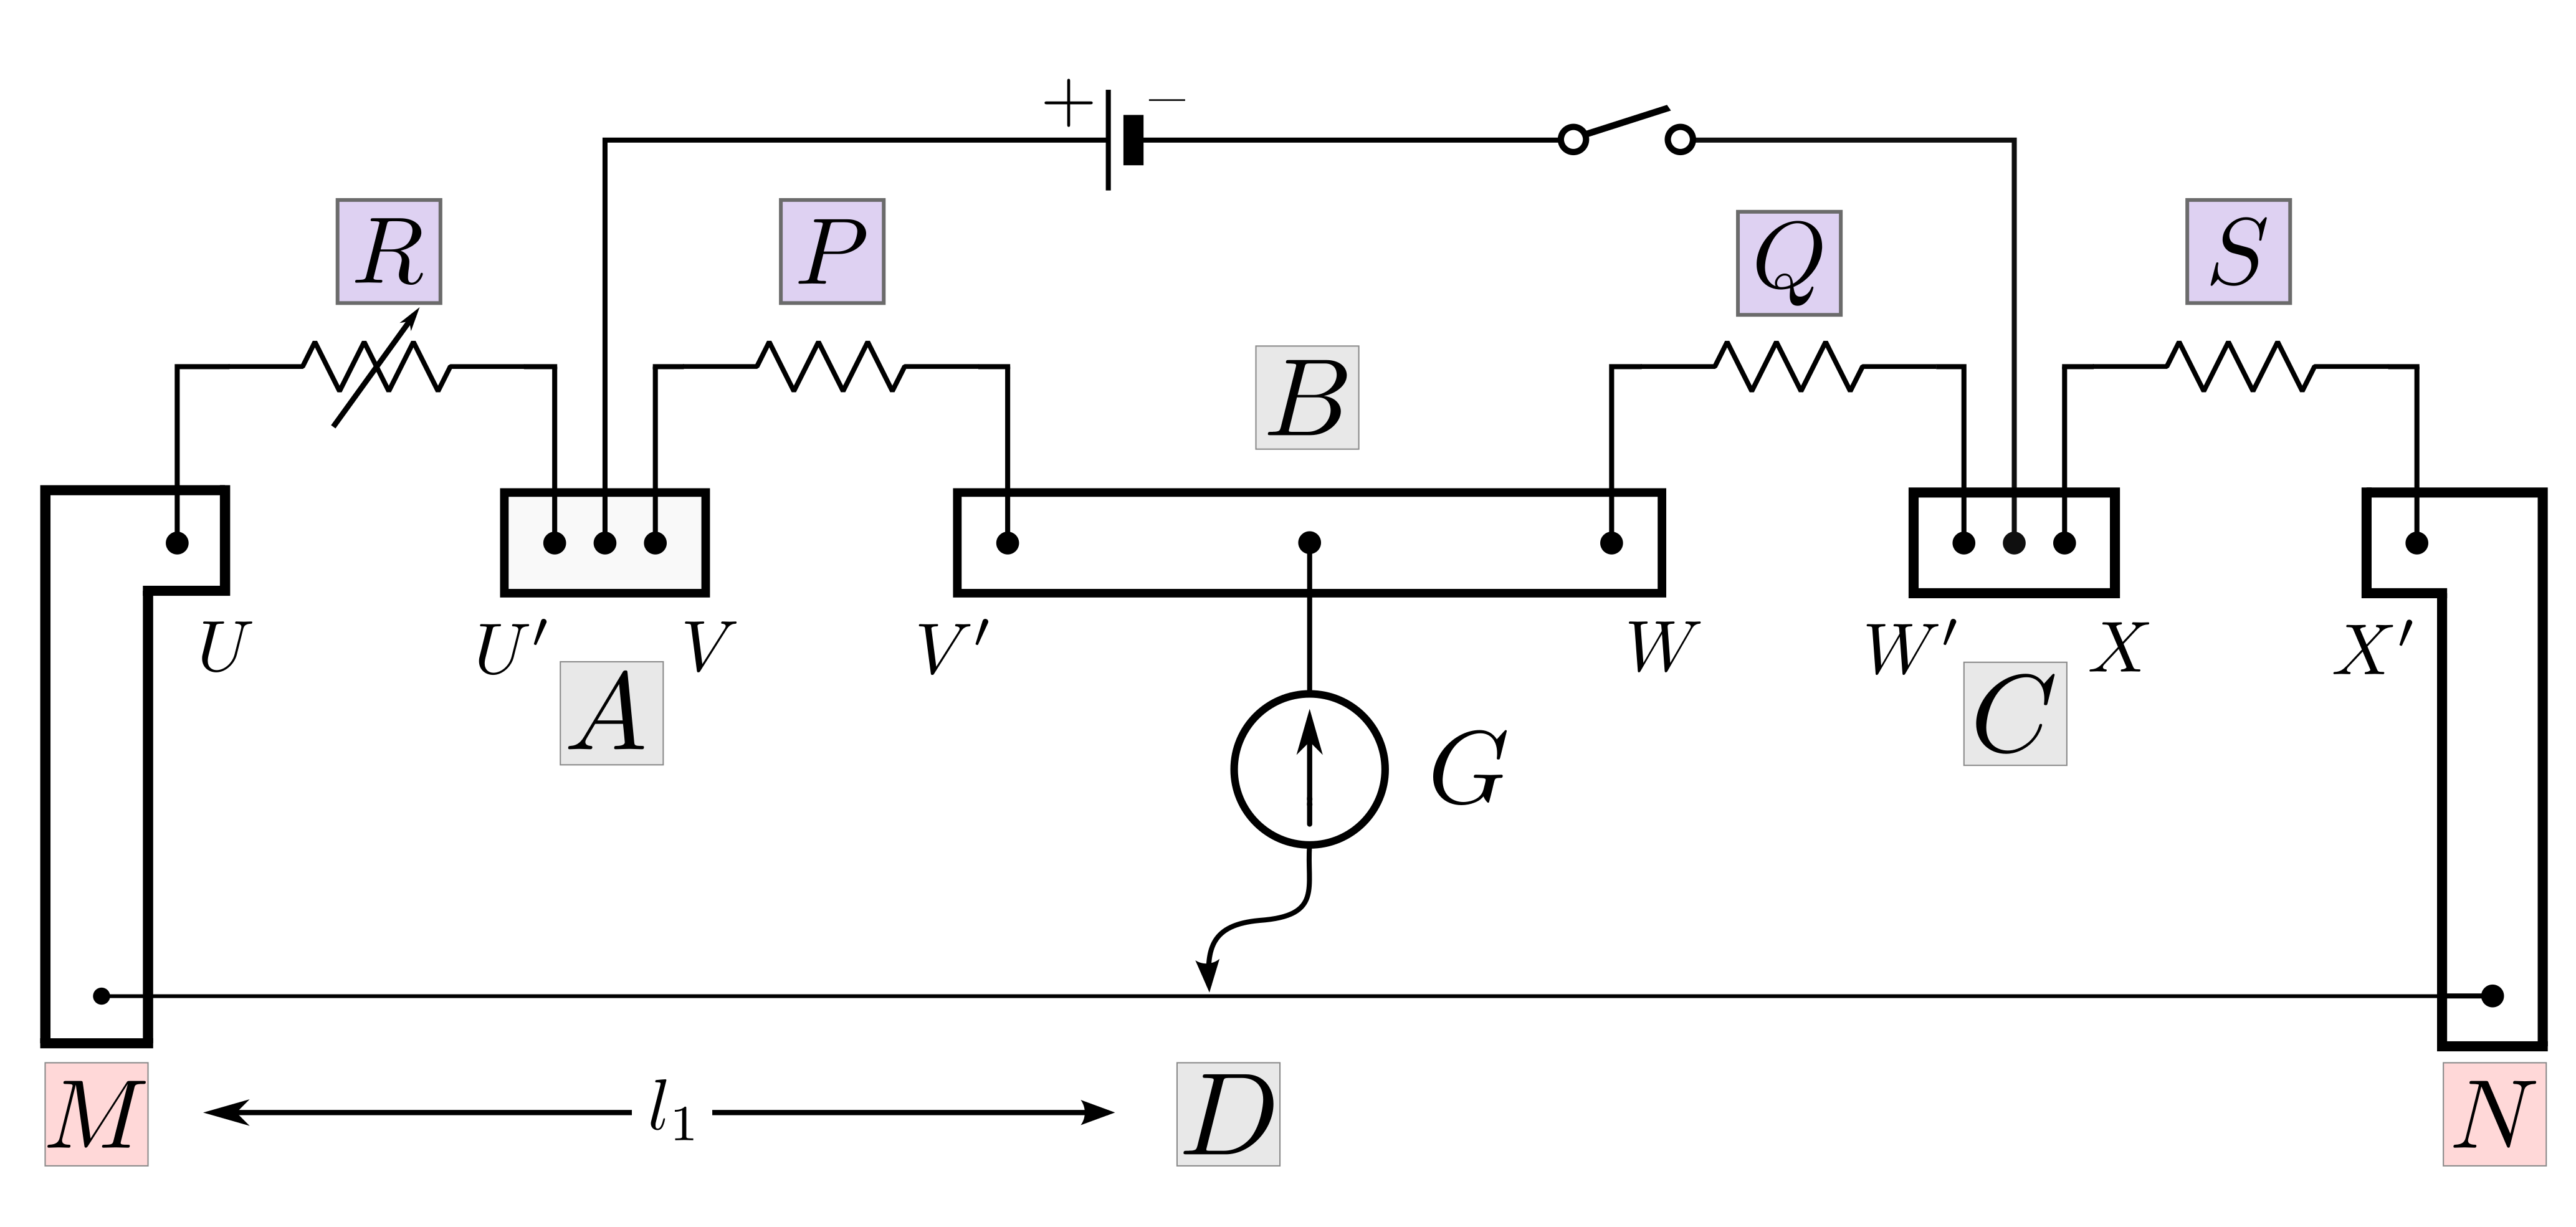
\includegraphics[width=\textwidth]{figs/carey.png}
    \caption{Schematic diagram of the Carey Foster bridge.}
    \label{fig:carey}
\end{figure}

The Carey Foster bridge with a circuit around it is illustrated in Figure (\ref{fig:carey}).
%The shaded part is a copper strip 
The bridge consists of a copper strip with four gaps (these act as four arms of a Wheatstone’s bridge). Two known resistances $P$ and $Q$ (equal and small) are connected in the inner gaps, $VV^{\prime}$ and $WW^{\prime}$. A null detector (galvanometer) is attached between the terminal $B$ and the jockey at $D$. A variable resistance box, $R$, with fractional resistances is placed in the outer gap at $UU^{\prime}$. The unknown (low) resistance, $S$, which is to be determined, is put in the 
outer gap at $XX^{\prime}$. A battery, a key, and a resistance box (if necessary) are connected between the terminals $A$ and $C$. A one metre long wire $MN$ of uniform resistance per unit length is mounted alongside a metre rod, and is soldered to the two ends of the copper strip. Since the jockey can be slid along the wire $MN$, the point $D$ can be anywhere between $M$ and $N$. It represents the position at which the null detector would register a value of 0. To locate this point, we tap the jockey over the wire. 

The wire, $MN$, is uniform and therefore, we may assume that it has a constant resistance per unit length, say, $r$ $\Omega$cm$^{-1}$. When the point $D$, located at some distance, $l_1$, from the end $M$ is chosen such that the null detector displays $0$, from the condition of a balanced Wheatstone bridge, we have, for the Carey Foster bridge 
\begin{equation}
\frac{P}{Q}=\frac{R+\delta_{1}+l_{1}r}{S+\delta_{2}+(100-l_{1})r}
\label{careyconfig1}
\end{equation}

Here, $\delta_{1}$ is the value of the resistance at the soldered junction, $M$, and $\delta_{2}$ is the value of the resistance at the junction $N$. These are end/contact resistances, which are unknown. Their presence would introduce an error in our measurement of $S$ if used the CF bridge directly as a Wheatstone bridge. So we would like to eliminate them. Notice that if we interchange $R$ and $S$ (the resistor $R$ is placed in gap $XX^{\prime}$, while the unknown resistance is now connected in gap $UU^{\prime}$), then, because $\delta_1$ and $\delta_2$ correspond to the same physical contacts, the balance equation becomes

\begin{equation}
\frac{P}{Q}=\frac{S+\delta_{1}+l_{2}r}{R+\delta_{2}+(100-l_{2})r}
\label{careyconfig2}
\end{equation}

Equations (\ref{careyconfig1}) and (\ref{careyconfig2}), together, yield the \textit{nice} (independent of end corrections) relation

\begin{equation}
S = R + (l_1-l_2)r
\label{CF}
\end{equation}

Clearly, by measuring $l_1$ and $l_2$ for an appropriate range of resistances, $R$, one can deduce the value of the unknown resistance, $S$ and also the resistance per unit length of the bridge wire. 

\begin{question}
\paragraph{Question:} Can we exchange the position of battery and the galvanometer? Which is the preferred arrangement and why?
\paragraph{Question:} Why does the procedure involve interchanging $R$ and $S$?
\paragraph{Question:} Draw the equivalent Wheatstone Bridge.
\paragraph{Question:} How is the Carey Foster an improvement over a standard Wheatstone bridge?
\paragraph{Question:} What is the largest unknown resistance that can be measured using a Carey Foster bridge?
\paragraph{Question:} In the derivation of the Equation (\ref{CF}), we eliminated $\delta_1$ and $\delta_2$ in favour of a relationships between $R$ and $S$. We can also use the two preceding balance equations to eliminate R and S, yielding an equation for $\delta_1 - \delta_2$. Derive this, explain why it might be useful.
\end{question}


\section*{Experimental Setup}

\subsection*{Apparatus}

\begin{enumerate}
\item A low voltage DC power supply
\item A Carey Foster bridge
\item Two fixed standard resistances (1 or 2 $\Omega$)
\item A fractional resistance box
\item A one-way key
\item A thick copper strip
\item An unknown low resistance ($S$)
\item A null detector (galvanometer)
\item Connecting wires.
\end{enumerate}


\subsection*{Precautions}
\begin{itemize}
    \item Clean all contacts thoroughly including %the battery terminals 
    the teeth of the alligator clips with sand paper.
    \item Make sure that enough wire is exposed while making connections, so that insulation does not come in between.
    \item Check each contact by tugging on the wire and ensuring that it does not loosen or come undone. 
    \item Arrange the elements of the circuit, so that it resembles your circuit diagram.
    \item While making the circuit think in terms of loops, not in terms of terminals. 
    \item Make sure there is a finite resistance in the circuit, \textit{before} the key is closed.
    \item Measure all balance lengths from the same side and on same scale.
\end{itemize}


\section*{Procedural Instructions}

\begin{imp}
Before starting observations, \textit{test} and \textit{debug} your circuit. Some common methods of debugging include checking the DC supply potential, checking continuity of your circuit using a multimeter. If there is no potential drop across a passive element, then check for continuity.
\end{imp}


\subsection*{Part A}

In this part, you will determine the apparent value of a small resistance.

\begin{enumerate}
    \item Make the connections as shown in the circuit diagram and connect the DC source. $S$ is the unknown resistance.
    \item Take out the zero resistance key from the resistance box ($R$) and note down the balance length ($l_1$). When determining the balance point, approach it from both sides and determine the range, if any, over which you get a null deflection. 
    \item Change the resistance in the box and find the new balance length.
    \item Interchange the position of the unknown resistance and the resistance box and repeat steps 1 to 3 to determine $l_2$.
    \item Tabulate $l_1 + l_2$.
    \item Plot a graph between $R$ and $l_1 -l_2$.
    \item Use this graph to determine the the resistance per unit length of the wire, and the apparent value of the unknown resistance.
\end{enumerate}

\subsection*{Part B}

In this part, you will determine a small correction to the above value. 
\begin{enumerate}
    \item Make the connections as shown in the circuit diagram and connect the DC source. ($S$ is a copper strip.)
    \item Take out the zero resistance plug from the resistance box ($R$) and note down the balance length ($l_1$). Approach the balance point from both sides, and if there is a range of readings corresponding to the null deflection, note the entire range. 
    \begin{tip}
        To make sure you are indeed at the balance point, infinitesimally moving the jockey, \textit{on either side}, should correspond to a small but finite current value on the galvanometer.
    \end{tip}
    \item Vary the resistance in the resistance box and find the new balance length.
    \item Interchange the position of the copper strip and the resistance box and repeat steps 1 to 3 to determine $l_2$.
    \item Tabulate $l_1 + l_2$. This is connected to the formula for $\delta_1 - \delta_2$ that you derived earlier.
    \begin{question}
    \paragraph{Question:} Why have you been asked to tabulate $l_1 + l_2$ even though it is not used in the calculations?
    \end{question}
    \item Plot a graph between $R$ and $l_1 -l_2$ on the same graph sheet as the one on which you plotted the readings in part A. 
    \item Examine the two lines carefully and check (i) whether they are parallel and (ii) what the apparent resistance of the copper strip is. 
    \item The unknown resistance in part A is not equal to the intercept but the difference between the intercepts of the lines in parts A and B. 
    
\end{enumerate}

\begin{question}
\paragraph{Question:} Why do the two lines -- from \textbf{Parts A} and \textbf{B} -- need to be parallel?
\paragraph{Question:} Explain the correction factor determined in \textbf{Part B}. 
\paragraph{Question:} Why is the graph with the unknown resistance alone enough to determine both the resistance per unit length and the unknown resistance?
\end{question}

\section*{References}

\begin{enumerate}
\item B. L. Worsnop, and H. T. Flint, \textit{Advanced Practical Physics for Students}.
\item Experiment 6, Measurement of Low Resistance using the Carey Foster Bridge, National Digital Repository (\textit{eGyanKosh})
\end{enumerate}


\newpage